\chapter{CSTR Model and Linearized Model Identification}

A prevalent modeling approach is to approximate the PDE (partial differential equation) model from the plug flow reactor
assumption into a set of ODEs (ordinary differential equations) using the idealization of the plug-flow reactor into a
sequence of continuous stirred tank reactors (CSTRs) (\cite{hsieh2011development}, and \cite{nova2014urea}). This
discretization requires at least 2 CSTRs to capture the system dynamics and causality, thereby increasing the model
order. Moreover, the reactions considered are generally confined to selected SCR and ASC reactions. The single CSTR
approach was first justified in \cite{devarakonda2008adequacy} and a nonlinear model was developed using these
assumptions, which was then linearized for feedback control design (\cite{devarakonda2009model}). With this model,
observers were designed to estimate the states corresponding to the catalyst's storage (\cite{ma2017observer},
\cite{jain2020term}). A method for detecting the catalyst's aging by observing the change in the maximum storage
capacity of the catalyst, modeled as an exponential function of temperature, was also proposed in \cite{ma2017observer}.
A common theme in these studies is the non-uniqueness in estimating the nonlinear parameters without a priori
constraints on the actual values. Moreover, these studies assume the availability of all the gaseous states at tail-pipe
to eliminate the effects of cross-sensitivity of the $NO_x$ sensors, which is not always the case in real-world
applications.

The present work aims to address these issues by proposing a reduced order model for the SCR-ASC system, whose parameter
estimation problem would be convex and implicitly considers the $NO_x$ sensor cross-sensitivity. Our approach is based
on the assumption that the detection of aging can be framed as a state/parameter estimation problem concerning the
concentration dynamics of the involved gases. Thus, in this paper, we present the development and validation of such a
reduced order linear model for the SCR-ASC system for diagnostics.

\section{Reduced Order Nonlinear Model}

The SCR-ASC system is a complex system with multiple reactions and transport.
The operating conditions and concentrations determine the selectivity of
reactants. The model development involves specific assumptions on these
characteristics which are aligned with the typical operating conditions and
system behavior. The CSTR assumption serves as the foundation for developing
the reaction flow model for SCR reactions. Based on the results of reduced
order modeling from previous studies including
\cite{devarakonda2008adequacy}, \cite{jain2023diagnostics}, we reduce the number
of reactions considered from the full set to three. Initially, we define the
reaction rate constants. Subsequently, we develop a comprehensive parametric
nonlinear model based on state definition of molar storage instead of the
typically used storage fraction state (\cite{nova2014urea}) for consistency with
experimental measurements and slight reduction in the complexity of
expressions.

\subsection{Reaction Kinetics}
We focus solely on the standard SCR reaction and assume all $NO_x$ in the
exhaust gas to be $NO$, given that commercially available $NO_x$ sensors cannot
differentiate between $NO$ and $NO_2$ (\cite{nova2014urea}). The slow SCR
reaction is not considered, as the exhaust's flow rate ensures that the slow
SCR reaction doesn't significantly contribute to the concentration of tail-pipe
exhaust components. Mass transfer is also neglected, suggesting that the
catalyst's chemical kinetics are reaction controlled, since the standard SCR
reaction rate surpasses the exhaust fluids' flow rate. We assume a $100\%$
nitrogen selectivity for ammonia oxidation both in SCR and in ASC
(\cite{jain2023diagnostics}).


Further, the reaction rates are assumed to be solely dependent on the gas-phase
concentrations of $NO_x$, $NH_3$, the adsorbed Ammonia, and the available
adsorption sites. To facilitate the control volume approach for mass balance,
concentration rates are converted into molar-rate. This is achieved using the
formula: $M_g = C_g V$, leading to $R_i = V r_i$. Rather than considering their
surface concentrations, the number of moles of the adsorbent is taken into
account directly. Additionally, a lower order Taylor approximation is employed
to model the temperature effects in the rate constant.

\begin{align*}
    k_i(\bar T + \delta T) &\approx k_i(\bar T) + p k_i(\bar T) \delta T\qquad
    \text{Where, }\quad   p = \frac{E_a}{R\bar{T}^2},\\
\end{align*}
\begin{align}
    \implies k_i(\delta T) &= \bar k_i + p \bar k_i \delta T
    \label{eqn::rate_approx}
\end{align}

\begin{enumerate}
\item Standard SCR reaction: $4 NH_3 (ads) + 4 NO + O_2 \longrightarrow 4 N_2 + 6 H_2O$
\begin{align*}
    R_1 &= k_1 V C_{NO} M_{NH_3} = k_1V C_{NO} \Theta \theta\\
    k_1 &= A_1 e^{\frac{-E_1}{RT}}
\end{align*}

\item AMOX with/without ASC: $4 NH_3 + 3 O_2 \longrightarrow 2 N_2 + 6 H_2O $
\begin{align*}
    R_3 &= k_3 M_{NH_3} = k_3 \Theta \theta\\
    k_3 &= A_3 e^{\frac{-E_3}{RT}}
\end{align*}

\item Ammonia Adsorption/Desorption: $NH_3 + \theta_{free} \longleftrightarrow NH_3(ads)$
\begin{enumerate}
\item Forward:
\begin{align*}
    R_{4F} &= k_{4F} V C_{NH_3} \lr{\Theta - M_{NH_3}}\\
    k_{4F} &= A_{4F} e^{\frac{-E_{4F}}{RT}}
\end{align*}
\item Reverse:
\begin{align*}
    R_{4R} &= k_{4R} M_{NH_3} = k_{4R} \Theta \theta \\
    k_{4R} &= A_{4R} e^{\frac{-E_{4R}}{RT}}
\end{align*}
\end{enumerate}
\end{enumerate}

\subsection{Urea Injection Model}

The actual input to the system is urea [from say, AdBlue ($32.5\%$ aqueous urea
solution) (\cite{nova2014urea})] injection that is converted to ammonia. This can be modelled by the following equation~(\ref{eqn::urea_inj}). The model is based on several assumptions related to the operating conditions. The evaporation of the urea-solutions is considered to be a significantly slower process than its decomposition into ammonia. This leads to the neglect of reaction kinetics, treating evaporation as a first order process in relation to the vapor pressure of the ammonia. The model also assumes a complete decoupling of the injection dynamics from other states. Furthermore, based on observations, the model assumes that urea is entirely converted to ammonia at the very upstream part of the SCR catalyst. These assumptions guide the reparametrization of the equation.
Let,
\begin{align*}
    x_4 &= C_{NH_3, in}, \quad b_u = 2 \frac{ \eta}{N_{urea}}, \quad \omega_u = \frac{1}{\tau}, \quad u_2 = u_{inj}
\end{align*}
\begin{equation}{\label{eqn::urea_inj}}
    \dot x_4 = - \omega_u x_4 +   \frac{\omega_u b_u}{f_v} u_{2}
\end{equation}

\subsection{Nonlinear Statespace Model}
We have the mass (moles of reactants in/out) balance from the CSTR assumption:
\begin{multline} \label{eqn::mass_balance}
    %===
    \bm{\dot C_{NO} \\  \dot C_{NH_3} \\ \dot M_{NH_3} } = b_v
    \bm{
        -R_1 - F C_{NO}\\
        -R_{4F} + R_{4R} - F C_{NH_3}\\
        R_{4F} - R_{4R} - R_1 - R_3
    }
    +
    f_vb_v \bm{1 & 0 \\ 0 & 1 \\ 0 & 0} \bm{ C_{NO, in} \\ C_{NH_3, in}}
    %===
\end{multline}
Let,
\begin{align*}
    \bm{x_1 \\ x_2 \\ x_3 \\ x_4} = \bm{C_{NO} \\ C_{NH_3} \\ M_{NH_3} \\ C_{NH_3, in}} \qquad &
    \bm{u_1 \\ u_2 } = \bm{C_{NO, in} \\ u_{inj}}
\end{align*}
We have the nonlinear statespace model as:
\begin{multline}
    \label{eqn::full_nonlinear}
     \bm{\dot x_1 \\
        \dot x_2\\
        \dot x_3\\
        \dot x_4} =
    \bm{
        -f_{13} x_1 x_3
        -g_1 x_1
        \\
        %===
        -g_2 x_2
        + f_{23} x_2 x_3
        + g_{23} x_3
        + f_{24} x_4
        \\
        %===
        -f_{32} x_2 x_3
        -g_3 x_3
        -f_{31} x_1 x_3
        + g_{32} x_2
        \\
        %===
        -g_4 x_4
    }
    + \bm{b_{11} & 0\\
          0     & 0\\
          0     & 0\\
          0     & b_{42}  }\bm{u_1 \\ u_2 }
\end{multline}
The lumped coefficients of the states are defined in the appendix of the chapter.

The sensor used for $NO_x$ measurement is sensitive to the ammonia in the
tailpipe. This cross-sensitivity $(\chi)$ can be incorporated into the model by writing
the output equation as:
\begin{align}\label{eqn::ctrl_out}
    y_1 &= x_1 + \chi x_2
\end{align}


\itbf{Note:} The above nonlinear state-space model is not parsimonious and identifiable with the available measurements. One way to get an identifiable model is to linearize the above nonlinear model and come up with lumped model parameters for I/O equations based on the available measurements. The remainder of this chapter focuses on this particular approach and the resulting aging signatures.


\section{Linear Model Development}

Utilizing small perturbations to linearize the model would explicitly reveal the dynamics' dependence on temperature and flow rate. Moreover, employing a linear model would broaden the range of tools available for estimator design.
The perturbation model would bring down the change in
temperature from exponential to algebraic form. We have the linearized model of the system:
\begin{multline}\label{eqn::lin_model}
    \bm{\delta \dot x_1 \\ \delta \dot x_2 \\ \delta \dot x_3 \\ \delta \dot x_4}
    = \underbrace{\bm{     a_{11} &
                    0 &
                    -\bar f_{13} \bar x_1 &
                    0 \\
                    %===
                    0 &
                    a_{22} &
                    a_{23} &
                    \bar f_{24} \\
                    %===
                    -\bar f_{31} \bar x_3 &
                    a_{32} &
                    a_{33} &
                    0 \\
                    %===
                    0 & 0 & 0 & -g_4
                    }}_A
    \bm{\delta x_1 \\ \delta x_2 \\ \delta x_3 \\ \delta x_4}
            + \underbrace{\bm{ \bar b_{11} &
                            0 &
                            \delta f_{13} \bar x_1 \bar x_3 &
                            b_{14}
                            \\
                        %===
                        0&
                        0 &
                        b_{23} &
                        b_{24} \\
                        %===
                        0&
                        0&
                        b_{33} &
                        0
                        \\
                        %===
                        0&
                        \bar b_{42}&
                        0&
                        \delta b_{42} \bar u_2
                        }}_B
    \bm{\delta u_1 \\ \delta u_2 \\ \delta T \\ \delta f_v}
\end{multline}
where the various symbols are defined in the appendix. Consequently, the output equation for the linearized model is given by:
\begin{equation}\label{eqn::lin_out}
    \delta y_1  = \delta x_1 + \chi \delta x_2
\end{equation}

\subsection{Input-to-State Transfer Function Model}
Since we have uncorrupted test-cell data for $NO_x$ and $NH_3$ and all the
inputs at any given time, part of the state-to-input transfer function matrix
can be estimated using this data. Transforming state-space model from
section-\ref{eqn::lin_model} into frequency domain, the model structure would
be:
\begin{align*}
    \bm{\delta x_1 \\ \delta x_2 \\ \hline \delta  x_3 \\ \delta x_4} &= \bm{G_{11} & G_{12} & G_{13} & G_{14}\\
                G_{21} & G_{22} & G_{23} & G_{24}\\
                \hline
                G_{31} & G_{32} & G_{33} & G_{34}\\
                G_{41} & G_{42} & G_{43} & G_{44}\\
    }
    \bm{\delta u_1 \\ \delta u_2 \\ \delta T \\ \delta f_v}
\end{align*}

With the given data, having $NO_x$ and $NH_3$ concentration measurements along
with all the inputs, $G_{1i}'s, G_{2i}'s$ can be estimated. Thus, the transfer function matrix that can be
identified using the available data is:
\begin{align*}
    G &= \bm{G_{11} & G_{12} & G_{13} & G_{14}\\
                G_{21} & G_{22} & G_{23} & G_{24}}
\end{align*}

Ignoring the actual output equation and using $C$ matrix that considers that the
first two states are measured, the input-to-state transfer function matrix is
given by:
\begin{align*}
    G &= C(sI-A)^{-1} B= \frac{1}{\norm{sI-A}} M B\\
    \text{Let, } M &= C \lr{\adj\lr{sI-A}} = \adj\lr{sI-A}[1:2, :]
\end{align*}
Thus only the first two rows of the adjoint of the $(sI-A)$ matrix are required
for computing the transfer function matrix.
Rewriting G as:
\begin{align*}
    G &= \frac{1}{D} \bm{N_{11} & N_{12} & N_{13} & N_{14}\\
                         N_{21} & N_{22} & N_{23} & N_{24}}
\end{align*}


% \subsubsection{Denominator Polynomial}
We have:
\begin{align*}
    D = |sI-A| &= \lr{g_4 + s} \times \underbrace{\lr{s^3 + d_2 s^2 + d_1 s + d_0}}_{D^{(3)}}
\end{align*}
Where,
\begin{align*}
    d_0 &= \left(\bar f_{13} - \bar f_{23}\right) \bar x_{3} + \bar f_{31} \bar x_{1} + \bar f_{32} \bar x_{2} + \bar g_{2} + \bar g_{3} + \bar g_{1}\\
    &= \left(\bar k_{4F} \bar x_{2} + \bar k_{4F}\right) \Theta + \left(\bar k_{1} - \bar k_{4F}\right) \bar x_{3} \\
    &\quad + \frac{V^{2} \bar k_{1} \bar x_{1} + V \bar k_{3} + V k_{4R} + 2 \bar f_v}{V}
\end{align*}

$d_1$ and $d_2$ are quadratic polynomials of nominal state values and
the storage capacity.

% \begin{align*}
%     d_2 &=- \bar f_{13} \bar f_{23} \bar x_{3}^{2} + \left(\bar f_{13} \bar f_{32} \bar x_{2} + \bar f_{13} \bar g_{2} + \bar f_{13} \bar g_{3} - \bar f_{23} \bar f_{31} \bar x_{1} - \bar f_{23} \bar g_{3} - \bar f_{23} \bar g_{1} + \bar f_{32} \bar g_{23}\right) \bar x_{3}\\
%     &\qquad  -  \bar f_{23} \bar g_{32} \bar x_{2} + \bar f_{31} \bar g_{2} \bar x_{1} + \bar f_{31} \bar g_{1} \bar x_{1} + \bar f_{32} \bar g_{2} \bar x_{2} + \bar f_{32} \bar g_{1} \bar x_{2} + \bar g_{2} \bar g_{3} + \bar g_{2} \bar g_{1} + \bar g_{3} \bar g_{1} - \bar g_{23} \bar g_{32}\\
%     &= \bar k_{4F}^{2} \bar x_{2} \Theta^{2} + \frac{V \bar k_{1} \bar k_{4F} \bar x_{2} + V \bar k_{1} \bar k_{4F} + \bar k_{4F} k_{4R}}{V} \Theta\bar x_{3} + \frac{V^{2} \bar k_{1} \bar k_{4F} \bar x_{1} - V^{2} \bar k_{4F}^{2} \bar x_{2} + V \bar k_{3} \bar k_{4F} + 2 \bar F \bar k_{4F} \bar x_{2} + \bar F \bar k_{4F}}{V} \Theta \\
%     &\qquad -  \bar k_{1} \bar k_{4F} \bar x_{3}^{2} + \frac{- V^{2} \bar k_{1} \bar k_{4F} \bar x_{1} + V \bar k_{1} \bar k_{3} + V \bar k_{1} k_{4R} - V \bar k_{3} \bar k_{4F} - V \bar k_{4F} k_{4R} + \bar F \bar k_{1} - \bar F \bar k_{4F}}{V} \bar x_{3} \\
%     &\qquad \qquad + \frac{2 V^{2} \bar F \bar k_{1} \bar x_{1} + 2 V \bar F \bar k_{3} + 2 V \bar F k_{4R} + \bar F^{2}}{V^{2}}
% \end{align*}
% \begin{align*}
%     d_3 &= \left(- \bar f_{13} \bar f_{23} \bar g_{3} + \bar f_{13} \bar f_{32} \bar g_{23}\right) \bar x_{3}^{2} \\
%     &\qquad + \left(- \bar f_{13} \bar f_{23} \bar g_{32} \bar x_{2} + \bar f_{13} \bar f_{32} \bar g_{2} \bar x_{2} + \bar f_{13} \bar g_{2} \bar g_{3} - \bar f_{13} \bar g_{23} \bar g_{32} - \bar f_{23} \bar f_{31} \bar g_{1} \bar x_{1} - \bar f_{23} \bar g_{3} \bar g_{1} + \bar f_{32} \bar g_{1} \bar g_{23}\right) \bar x_{3} \\
%     &\qquad \qquad -  \bar f_{23} \bar g_{1} \bar g_{32} \bar x_{2} + \bar f_{31} \bar g_{2} \bar g_{1} \bar x_{1} + \bar f_{32} \bar g_{2} \bar g_{1} \bar x_{2} + \bar g_{2} \bar g_{3} \bar g_{1} - \bar g_{1} \bar g_{23} \bar g_{32}\\
%     &=  \bar k_{1} \bar k_{4F}^{2} \bar x_{2} \Theta^{2}\bar x_{3} + \frac{\bar F \bar k_{4F}^{2} \bar x_{2}}{V} \Theta^{2} + \frac{\bar k_{1} \bar k_{4F} k_{4R}}{V} \Theta\bar x_{3}^{2} + \frac{- V^{3} \bar k_{1} \bar k_{4F}^{2} \bar x_{2} + V^{2} \bar k_{1} \bar k_{3} \bar k_{4F} + V \bar F \bar k_{1} \bar k_{4F} \bar x_{2} + \bar F \bar k_{4F} k_{4R}}{V^{2}} \Theta\bar x_{3} \\
%     & \qquad + \frac{V^{2} \bar F \bar k_{1} \bar k_{4F} \bar x_{1} - V^{2} \bar F \bar k_{4F}^{2} \bar x_{2} + V \bar F \bar k_{3} \bar k_{4F} + \bar F^{2} \bar k_{4F} \bar x_{2}}{V^{2}} \Theta + \left(- \bar k_{1} \bar k_{3} \bar k_{4F} - \bar k_{1} \bar k_{4F} k_{4R}\right) \bar x_{3}^{2} \\
%     &\qquad \qquad + \frac{- V \bar F \bar k_{1} \bar k_{4F} \bar x_{1} + \bar F \bar k_{1} \bar k_{3} + \bar F \bar k_{1} k_{4R} - \bar F \bar k_{3} \bar k_{4F} - \bar F \bar k_{4F} k_{4R}}{V} \bar x_{3} + \frac{V \bar F^{2} \bar k_{1} \bar x_{1} + \bar F^{2} \bar k_{3} + \bar F^{2} k_{4R}}{V^{2}}
% \end{align*}

% \subsubsection{Numerator Matrix}
We have the numerator matrix of the transfer function matrix:
\begin{align*}
    N &= \bm{N_1 \\ N_2} = \bm{N_{11} & N_{12} & N_{13} & N_{14}\\
             N_{21} & N_{22} & N_{23} & N_{24}} = M B
\end{align*}

Where, $M$ is the first two rows of the adjoint matrix of $sI-A$. Calculating
the expressions for each of the elements of $N$ matrix symbolically:

\begin{minipage}{0.49\textwidth}
 \begin{align*}
    N_{11} &= (s + g_4)(n_{11_2} s^2 + n_{11_1} s + n_{11_0})\\
    %===
    N_{12} &= \bar b_{42} \bar f_{13} \bar f_{24} \bar x_{1} \left(\bar f_{32} \bar x_{3} - \bar g_{32}\right) \\
    &= \frac{\Theta \bar k_{1} \bar k_{4F} \bar x_{1} \omega_{u} b_{u} \left(- V + \bar x_{3}\right)}{V}\\
    %===
    N_{13} &= (s + g_4)(n_{13_2} s^2 + n_{13_1} s + n_{13_0})\\
    %===
    N_{14} &= n_{14_3} s^3 + n_{14_2} s^2 + n_{14_1} s + n_{14_0}\\
 \end{align*}
\end{minipage}
\begin{minipage}{0.49\textwidth}
 \begin{align*}
    %===
    N_{21} &= - \bar b_{11} \bar f_{31} \bar x_{3} \left(g_{4} + s\right) \left(\bar f_{23} \bar x_{2} + \bar g_{23}\right) \\
    %===
    N_{22} &= n_{22_2} s^2 + n_{22_1} s + n_{22_0}\\
    %===
    N_{23} &= (s + g_4)(n_{23_2} s^2 + n_{23_1} s + n_{23_0})\\
    %===
    N_{24} &= n_{14_3} s^3 + n_{14_2} s^2 + n_{14_1} s + n_{14_0}\\
\end{align*}
\end{minipage}

\itbf{Pole-Zero Cancellation:} Symbolic computations reveal that $s + g_4$ is
the common factor among all the numerator polynomials and the denominator. This
gets cancelled, removing all the direct effects of urea-dosing dynamics on
$\delta x_1, \delta x_2$ from temperature and $NO_x$ inputs. The flow rate
interacts with the urea-dosing dynamics as it affects the urea decomposition rate.

From previous calculations, we can arrive at a general structure for the
transfer function matrices. Let $^{(i)}$ denote the polynomial order of the
expression in $'s'$ (Laplace variable).

Thus,
\begin{align} \label{eqn::I2S_tf}
    G &= \bm{\frac{N_{11}^{(2)}}{D^{(3)}} &
             \frac{N_{12}^{(0)}}{\lrb{(s+g_4) D^{(3)}}} &
             \frac{N_{13}^{(2)}}{D^{(3)}} &
             \frac{N_{14}^{(3)}}{\lrb{(s+g_4)D^{(3)}}}
             \\
             \frac{N_{21}^{(0)}}{D^{(3)}} &
             \frac{N_{22}^{(2)}}{\lrb{(s+g_4)D^{(3)}}} &
             \frac{N_{23}^{(2)}}{D^{(3)}} &
             \frac{N_{24}^{(3)}}{\lrb{(s+g_4) D^{(3)}}}
    }
\end{align}

The above model structure information can be used to identify the transfer
function model for the linearized system. The transfer function model can be
converted into regression form and least-squares optimization can be used to
identify the model parameters. The regression form of the model would be:

\begin{align} \label{eqn::I2S_regression_form}
    \bm{\frac{d^4 x_1}{dt^4}\\
        \frac{d^4 x_2}{dt^4}}
    &= \bm{\pmb \phi_D(x_1)
            & \pmb \phi_{N_1}
            & \pmb 0\\
            \pmb \phi_D(x_2)
            & \pmb 0
            & \pmb \phi_{N_2}}
        \bm{\pmb \theta_D \\ \pmb \theta_{N_1} \\ \pmb \theta_{N_2}}
\end{align}


\subsection{Input-Output Transfer Function Model}
The input-output transfer function model for the linearized system can be
derived from the input-to-state transfer function (\ref{eqn::I2S_tf}) model
using the output equation~(\ref{eqn::lin_out})
\begin{align}
    G_y &= \frac{1}{D} \bm{N_1 + \chi N_2}  \label{eqn::I2O_tf}
\end{align}

The above transfer function model will have a regression form similiar to
eqation~(\ref{eqn::I2S_regression_form}) with the following structure:
\begin{align} \label{eqn::I2O_regression_form}
    \frac{d^4 y_1}{dt^4} &= \bm{\pmb \phi_D(y_1) & \pmb \phi_{N_y}} \bm{\pmb \theta_D \\ \pmb \theta_{N_y}}
\end{align}

%\subsection{Remarks on the linearized model}

Several insights can be drawn from the structure of the $A$ and $B$ matrices in
the linearized model. From the $A$ matrix, it is observed that the change in
$NO_x$ concentration $(\delta x_1)$ influences only the catalyst storage
dynamics of ammonia $(\delta x_3)$, and itself. Urea injection $(\delta x_4)$
similarly only impacts the ammonia concentration dynamics $(\delta x_2)$, and
itself. The dynamics of urea injection are solely affected by its
concentration, independent of other states. A strong coupling is also noted
between ammonia storage and ammonia concentration. Turning to the $B$ matrix,
the $NO_x$ input $(u_1)$ is seen to affect only the $NO_x$ concentration, not
any other state. The dynamics of urea injection $(\delta x_4)$ are found to be
independent of both temperature and $NO_x$ input $(u_1)$, relying only on the
injection rate $(\delta u_2)$ and the flow rate $(\delta f_v)$. Lastly, the
catalyst's ammonia storage is observed to depend exclusively on temperature
change, unaffected by other factors.


\section{Linear Model Identification}
The linearized model derived previously can be used for model parameter
identification. The idea is to identify the lumped linear model parameters and
then use this information to arrive at the estimates for the relevant parameters
for prediction/aging-factor estimation purposes.

The test-cell data used for the identification of the linear model includes measurements of all the inputs, output and the first two states of the
model. Thus, for model parameter estimation, the following regression form that
combines equations~(\ref{eqn::I2S_regression_form}) and
(\ref{eqn::I2O_regression_form}) can be used:
\begin{align}\label{eqn::regression_form}
    \bm{\frac{d^4 x_1}{dt^4}\\
        \frac{d^4 x_2}{dt^4}\\
        \frac{d^4 y_1}{dt^4}}
    &= \bm{\pmb \phi_D(x_1)
            & \pmb \phi_{N_1}
            & \pmb 0
            & \pmb 0\\
            \pmb \phi_D(x_2)
            & \pmb 0
            & \pmb \phi_{N_2}
            &\pmb 0\\
            \pmb \phi_D(y_1)
            & \pmb 0
            & \pmb 0
            & \pmb \phi_{N_y}}
        \bm{\pmb \theta_D \\ \pmb \theta_{N_1} \\ \pmb \theta_{N_2}\\ \pmb \theta_{N_y}}
\end{align}

The higher-order derivatives are computed using Savitzky-Golay FIR filter
(\cite{schafer2011savitzky}) with break frequency around $0.3\, Hz$, with any
lag being compensated for by shifting and truncating the data. The choice of
break frequency is based on the frequency response of the test-cell data.
The model comprises 45 parameters that need to be estimated, derived
from three independent measurement channels. Linear least-squares method
would result in the minimum variance and unbiased parameter estimates for this
model structure (\cite{lennart1999system}). A nonlinear inequality constraint
based on Routh-Hurwitz criterion is used to ensure the stability of the common
denominator polynomial.
%===============================================================================
\subsection{Model structure validation and parameter estimation}

\begin{figure}[h]
    \centering
    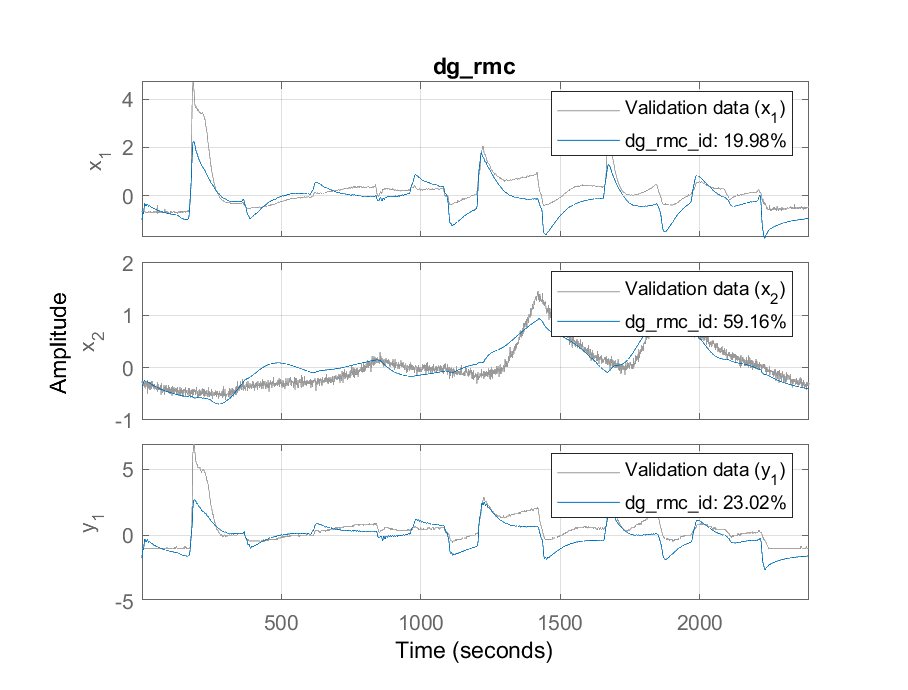
\includegraphics[width=0.7\textwidth]{Part3/figs/4_figs/dg_valid.eps}
    \caption{Comparison of the identified model with the normalized RMC test data for degreened catalyst}
    \label{fig:dg_comp}
\end{figure}

\begin{figure}[h]
    \centering
    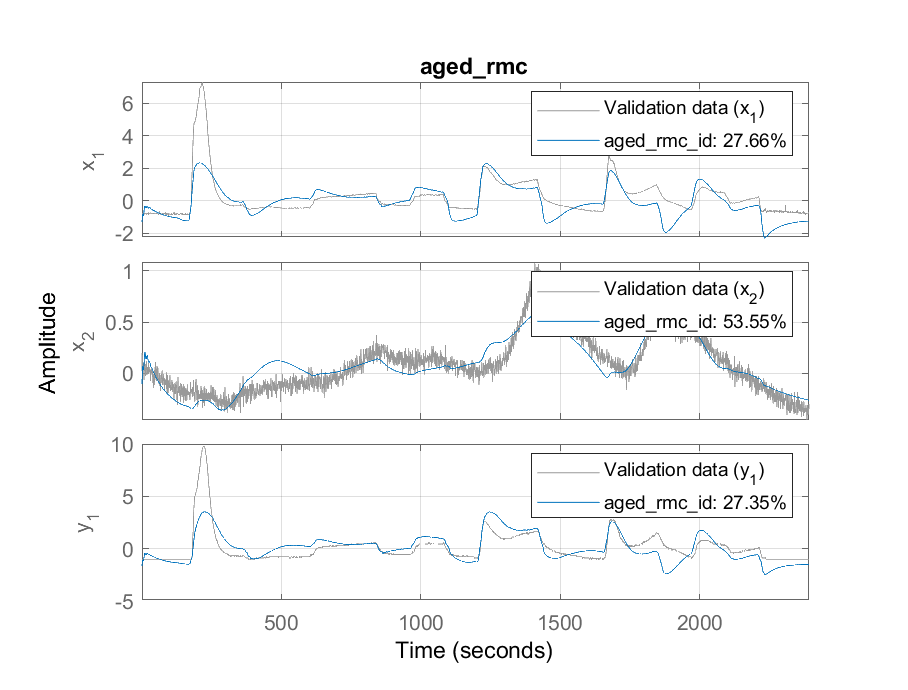
\includegraphics[width=0.7\textwidth]{Part3/figs/4_figs/aged_valid.eps}
    \caption{Comparison of the identified model with the normalized RMC test data for aged catalyst}
    \label{fig:ag_comp}
\end{figure}

Test-cell data (sampled at $5\, Hz$) from three tests (Ramped Mode Cycle (RMC),
hot and cold Federal Test Procedure (FTP))
on both aged and degreened catalysts is used for model structure validation and
model parameter estimation. The validation is done by comparing the test-cell
(experimental) response with the simulation using the estimated model
parameters (Figures~\ref{fig:dg_comp} and \ref{fig:ag_comp}). $\%fit$ is
calculated on the entire time-series of experimental data and simulation to arrive
at the goodness of fit for the model structure. This indicates the percent of
the output data that is captured by the model structure.

As shown in Table~\ref{tab:pfit}, the model structure fits reasonably well
in the cases of RMC and hot FTP data sets. The linear model structure doesn't
capture the dynamics in cold FTP case as the temperature fluctuations are
greater than $\pm 50\, ^0 C$ ($\approx \pm 100\, ^0C$) for which the linear
approximation of the rate constants (\ref{eqn::rate_approx}) is not valid.


\begin{table}[h]
\caption{Model structure validation for test data using prediction error} \label{tab:pfit}
    \begin{center}
    \begin{tabular}{| l | r l | r l |}
        \hline
 & \textbf{Aged} & \textbf{Data} & \textbf{Degreened} & \textbf{Data}
\\
\textbf{Test} & $NO_x$    & $NH_3$    &  $NO_x$   & $NH_3$   \\
& $(\%fit)$ & $(\%fit)$ &  $(\%fit)$& $(\%fit)$\\ \hline
        RMC           & $27.66$ & $53.55$ & $19.98$ & $59.16$ \\ \hline
        hot FTP       & $7.105$ & $38.31$ & $7.385$ & $56$\\ \hline
        cold FTP*      & $23.19$ & $-32.88$& $23.24$ & $-1.77$\\ \hline
\end{tabular}
    \end{center}
\itbf{Note}: $\%fit = 100 \times \lr{1 - \frac{\norm{Y- \hat Y}}{\norm{Y -
mean(Y)}}}$ is the percentage of the measured output that was explained by the
model.\\
*Cold FTP data set is not in the operating range of the linearized model.
\end{table}


The model structure can be further utilized for characterizing catalyst aging
and for diagnostic purposes. Specifically, the values of $N_{12}/\bar x$ could
be a good indicator of the catalyst aging if its value is statistically
different for aged and degreened catalysts. This value for the data sets is
tabulated in Table~\ref{tab:N12_comp}. The statistical validation of
difference in the value of $N_{12}/\bar x$ for aged and degreened catalysts is left for future work.

\begin{table}[h]
\caption{Comparison of $N_{12}/\bar x$ estimate for aged and degreened
    catalysts in test data} \label{tab:N12_comp}
    \centering
    \begin{tabular}{|l|c|c|}
        \hline
        \textbf{Test Data} & \textbf{Aged Data} & \textbf{Degreened Data}\\ \hline
        RMC                & 0.0116        & 0.0034 \\ \hline
        hot FTP            & 0.0099        & 0.0030 \\ \hline
        cold FTP           & -0.0281       & -0.0241 \\ \hline
    \end{tabular}
\end{table}

\section{Remarks}
The work showcases the effectiveness of using a linearized model dynamics of
an SCR-ASC system for diagnostics. The model, derived from first principles and
grounded on reasonable assumptions, provides a simplified yet insightful
perspective on the SCR system dynamics. This simplification facilitates the
application of system identification methods to obtain unique parameter values.
The model's validity is confirmed using experimental data from test-cell under
specific operating conditions. A particular focus is placed on input gain from
urea dosing to tail-pipe $NO_x$ ($N_{12}$), which is a monotonic function of
catalyst's nominal and total molar storage capacity, proving valuable for
monitoring catalyst aging.

% \section{List of Symbols}

\begin{table}[H]
    \begin{tabular}{r c l}
        \textbf{\underline{Variable}} & & \textbf{\underline{Description}}\\
        $A_1$ & & Pre-exponential factor for SCR reaction\\
        $A_3$ & & Pre-exponential factor for AMOX reaction\\
        $A_{4F}$ & & Pre-exponential factor for ammonia adsorption\\
        $A_{4R}$ & & Pre-exponential factor for ammonia desorption\\
        $b_u$ & & Urea injection parameter\\
        $C_{\bullet}^{*} \,or \,  [\bullet]^{*}$ & &
        Concentration of species ($\bullet$) \\
        $M_{\bullet}^{*} \, or \,  \{\bullet\}^{*}$ & &
        Moles of species ($\bullet$) at inlet, outlet or adsorbed\\
        $E_1$ & & Activation energy for SCR reaction\\
        $E_3$ & & Activation energy for AMOX reaction\\
        $E_{4F}$ & & Activation energy for ammonia adsorption\\
        $E_{4R}$ & & Activation energy for ammonia desorption\\
        $F$ & & Exhaust Mass Flow Rate\\
        $f_v$ & & Exhaust Volume Flow Rate $\lr{=\frac{F}{\rho} = \frac{FT}{\mu}}$\\
        $\rho$ & & Density of the exhaust $\lr{=\frac{\mu}{T}}$\\
        $V$ & & Volume of the reactor\\
        $b_v$ & & Reciprocal of the reactor volume $=\frac{1}{V}$\\
        $k_1$ & & Rate constant for SCR reaction\\
        $k_3$ & & Rate constant for AMOX reaction\\
        $k_{4F}$ & & Rate constant for ammonia adsorption\\
        $k_{4R}$ & & Rate constant for ammonia desorption\\
        $M_{NH_3}$ & & Moles ammonia adsorbed\\
        $\tau$ & & Time constant of urea decomposition\\
        $u_{inj}$ & & Mass injection rate of the AdBlue solution\\
        $\eta$    & & Mass fraction of urea in the solution\\
        $N_{urea}$ & &Atomic number of urea\\
        $\Theta$ & & Moles of available adsorption sites\\
        $R_i$ & & Molar rate of reaction $i$\\
        $r_i$ & & Rate of reaction $i$\\
        RMC & & Ramped mode cycle\\
        FTP & & Federal test procedure
    \end{tabular}
\end{table}

\section*{Appendix}
\subsection*{Identified transfer function model parameters}
\begin{minipage}{0.49\textwidth}
\begin{align*}
    \footnotesize
    &\text{Aged Model}\\
    D &= s^4 + 0.381 s^3 + 0.540 s^2 + 0.111 s + 0.004\\
    N_{11} &= 0.194 s^3 + 0.18 s^2 + 0.245 s + 0.004\\
    N_{12} &= 0.004\\
    N_{13} &= 16.01 s^3 - 0.338 s^2 - 2.023 s  - 0.011\\
    N_{14} &= 0.092 s^3 + 0.064 s^2 + 0.003 s - 0.001\\
    N_{21} &=  0.010 s - 0.004\\
    N_{22} &= 0.003 s^2 + 0.002 s - 0.001\\
    N_{23} &= 0.313 s^3 + 1.196 s^2 + 0.160 s + 0.007\\
    N_{24} &= 0.047 s^3 + 0.002 s^2 + 0.017 s + 0.004
\end{align*}
\end{minipage}
\begin{minipage}{0.49\textwidth}
\begin{align*}
    \footnotesize
    &\text{Degreened Model}\\
    D &= s^4 + 0.396 s^3 + 0.531 s^2 + 0.115 s + 0.006\\
    N_{11} &= 0.148 s^3 - 0.048 s^2 + 0.165 s + 0.008\\
    N_{12} &= 0.001\\
    N_{13} &= 2.661 s^3 + 2.359 s^2 - 1.819 s - 0.010\\
    N_{14} &= 0.106 s^3 + 0.056 s^2 + 0.026 s - 0.001\\
    N_{21} &= 0.0126 s - 0.004\\
    N_{22} &= -0.001 s^2 + 0.001 s + 0.001\\
    N_{23} &= -0.101 s^3 - 0.220 s^2 - 0.190 s  + 0.016\\
    N_{24} &= 0.0004 s^3 - 0.003 s^2 + 0.003 s + 0.003
\end{align*}
\end{minipage}

\subsection*{Regressor Vectors}
The following are the regressor vectors used for model parameter identification.
\begin{figure}[H]
\begin{minipage}{0.45\columnwidth}
    \begin{align*}
        \footnotesize
        \pmb \phi_{N_1} &= \bm{\phi_{N_1}^{u_1} & \phi_{N_1}^{u_2} & \phi_{N_1}^T & \phi_{N_1}^F}\\
       & \phi_{N_1}^{u_1} = \bm{\dddot u_1& \ddot u_1& \dot u_1&  u_1}\\
       & \phi_{N_1}^{u_2} = \bm{u_2}\\
       & \phi_{N_1}^T = \bm{\dddot T& \ddot T& \dot T&  T}\\
       & \phi_{N_1}^F = \bm{\dddot f_v& \ddot f_v& \dot f_v&  f_v}\\
       %===
        \pmb \phi_{N_2} &= \bm{\phi_{N_2}^{u_1} & \phi_{N_2}^{u_2} & \phi_{N_2}^T & \phi_{N_2}^F}\\
       & \phi_{N_2}^{u_1} = \bm{\dot u_1 & u_1}\\
       & \phi_{N_2}^{u_2} = \bm{\ddot u_2& \dot u_2&  u_2}\\
       & \phi_{N_2}^T = \bm{\dddot T& \ddot T& \dot T&  T}\\
       & \phi_{N_2}^F = \bm{\dddot f_v& \ddot f_v& \dot f_v&  f_v}
       %===
    \end{align*}
\end{minipage}
\begin{minipage}{0.45\columnwidth}
    \begin{align*}
        \footnotesize
        \pmb \phi_D(x) &= \bm{-\dddot x& -\ddot x& -\dot x& - x}\\
        %====
         \pmb \phi_{N_y} &= \bm{\phi_{N_y}^{u_1} & \phi_{N_y}^{u_2} & \phi_{N_y}^T & \phi_{N_y}^F}\\
       & \phi_{N_y}^{u_1} = \bm{\dddot u_1& \ddot u_1& \dot u_1&  u_1}\\
       & \phi_{N_y}^{u_2} = \bm{\dot u_2&  u_2}\\
       & \phi_{N_y}^T = \bm{\dddot T& \ddot T& \dot T&  T}\\
       & \phi_{N_y}^F = \bm{\dddot f_v& \ddot f_v& \dot f_v&  f_v}
    \end{align*}
\end{minipage}
\end{figure}

\subsection*{Model Parameter Definitions}
\begin{itemize}
\item Parameters of the nonlinear model (equation~\ref{eqn::full_nonlinear})
\begin{align*}
    \footnotesize
    &\mat{
    \\f_{13} &=& k_1
    \\f_{23} &=& k_{4F}
    \\f_{32} &=& k_{4F} \Theta
    \\f_{31} &=& k_1 V
    \\f_{24} &=& b_v f_v
    \\b_{11} &=& b_v f_v
    },
    \qquad \qquad \qquad
    \mat{
    \\ g_1    &=& b_v f_v
    \\ g_2    &=& b_v f_v + k_{4F} \Theta
    \\ g_{3}  &=& k_{4R}+k_3
    \\ g_{23} &=& k_{4R} V^{-1}
    \\ g_{32} &=& k_{4F} V \Theta
    \\ g_4 &=& \omega_u
    \\ b_{42} &=& \frac{\omega_u b_u}{f_v}
    }
\end{align*}
%===============================================================================
\item Parameters of the linear model (equation~\ref{eqn::lin_model})

\begin{minipage}{0.49 \textwidth}
\begin{align*}
    \footnotesize
    a_{11} &= -\lr{ \bar f_{13} \bar x_3 + \bar g_1 } \\
    a_{22} &= \lr{ -\bar g_2 + \bar f_{23} \bar x_3 } \\
    a_{23} &= \lr{\bar f_{23} \bar x_2 + \bar g_{23}} \\
    a_{32} &= \lr{-\bar f_{32} \bar x_3 + \bar g_{32} } \\
    a_{33} &= \lr{-\bar f_{32} \bar x_2 - \bar g_3 - \bar f_{31} \bar x_1}  \\
    b_{23} &= -\delta g_{2_T} \bar x_2 + \delta f_{23} \bar x_2 \bar x_3 + \delta g_{23} \bar x_3 \\
    b_{33} &= -\delta f_{32} \bar x_2 \bar x_3 - \delta g_3 \bar x_3 - \delta f_{31} \bar x_1 \bar x_3 + \delta g_{32} \bar x_2 \\
    b_{14} &= \lr{\delta b_{11} \bar u_1- \delta g_1 \bar x_1} \\
    b_{24} &= \lr{-\delta g_{2_F} \bar x_2 + \delta f_{24} \bar x_4 }\\
    %===
\end{align*}
\end{minipage}
\begin{minipage}{0.49\textwidth}
\begin{align*}
    \footnotesize
    %===
    \bar f_{13} &= \bar k_{1}, \quad
    \delta f_{13}  = \lr{ p_{1} \bar k_{1} } \\
    %===
    \bar f_{23} &= \bar k_{4F}, \quad
    \delta f_{23} = \lr{ p_{4F} \bar k_{4F} } \\
    %===
    \bar f_{32} &= \bar k_{4F} \Theta, \quad
    \delta f_{32}  = \lr{ p_{4F}  \bar k_{4F} \Theta }
    \\
    \bar f_{31} &= \bar k_1 V, \quad
    \delta f_{31}  = \lr{ p_1 \bar k_1 V }
    \\
    \bar f_{24} &= b_v \bar f_v,
    \quad
    \delta f_{24}  = b_v
    \\
   \bar g_1 &= b_v \bar f_v,
    \quad
    \delta g_1  = b_v
    \\
   \bar g_2 &= b_v \bar f_v + \bar k_{4F} \Theta,
    \quad
    (\delta g_{2_F} , \delta g_{2_T}) = (b_v,  \lr{ p_{4F}  \bar k_{4F}  \Theta })
    \\
    \bar g_3 &= \bar k_{4R} + \bar k_3,
    \quad
    \delta g_3 = \lr{ p_{4R} \bar k_{4R} + p_3 \bar k_3}
    \\
    \bar g_{23} &= \bar k_{4R} b_v,
    \quad
    \delta g_{23}  = \lr{ p_{4R} \bar k_{4R} b_v }
    \\
    \bar g_{32} &= \bar k_{4F} V \Theta,
    \quad
    \delta g_{32}  = \lr{ p_{4F} \bar k_{4F} V \Theta }
    \\
    \bar b_{11} &= b_v \bar f_v,
    \quad
    \delta b_{11}  = b_v
    \\
    \bar b_{42} &= \frac{\omega_u b_u}{\bar f_v},
    \quad
    \delta b_{42}  = -\lr{\frac{\omega_u b_u}{\bar f_v^2}}
\end{align*}
\end{minipage}

\end{itemize}


